\section{Make PDF}
\label{seq:GanttMakePDF}
\subsection{Basic course}
Il client entra nella pagina relativa al diagramma Gantt e clicca sulla 
funzionalit\`a ''Make PDF''. Il sistema costruisce un oggetto in questo modo:
\begin{itemize}
  \item invoca lo use case \ref{seq:GanttMakeLeftColumn} per creare la
  colonna a sinistra.
  \item invoca lo use case \ref{seq:GanttRightRepresentation} per creare
  la rappresentazione nel tempo (colonna destra del diagramma).
\end{itemize}
Il sistema invio la pagina di risposta al client, aggiungendo accanto ai
pulsanti di reporting una icona per permettere il download del file generato.  

\subsection{Alternative course}
\begin{description}
\item[nessuna]
\end{description}

\subsection{UML use case diagram}
\begin{figure}[h] \centering
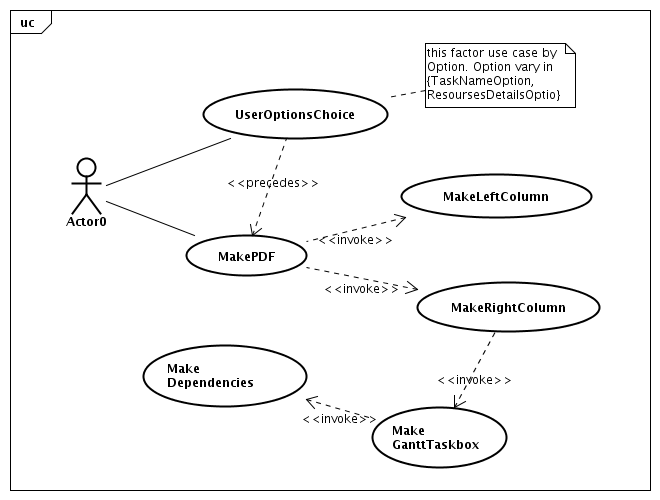
\includegraphics[width=0.8\textwidth]{Gantt/img/MakePDF.png} 
\end{figure}